%; whizzy chapter
% -initex iniptex -latex platex -format platex -bibtex jbibtex -fmt fmt
% 以上 whizzytex を使用する場合の設定。

%     Kansai Debian Meeting resources
%     Copyright (C) 2007 Takaya Yamashita
%     Thank you for Tokyo Debian Meeting resources

%     This program is free software; you can redistribute it and/or modify
%     it under the terms of the GNU General Public License as published by
%     the Free Software Foundation; either version 2 of the License, or
%     (at your option) any later version.

%     This program is distributed in the hope that it will be useful,
%     but WITHOUT ANY WARRANTY; without even the implied warranty of
%     MERCHANTABILITY or FITNESS FOR A PARTICULAR PURPOSE.  See the
%     GNU General Public License for more details.

%     You should have received a copy of the GNU General Public License
%     along with this program; if not, write to the Free Software
%     Foundation, Inc., 51 Franklin St, Fifth Floor, Boston, MA  02110-1301 USA

%  preview (shell-command (concat "evince " (replace-regexp-in-string "tex$" "pdf"(buffer-file-name)) "&"))
% 画像ファイルを処理するためにはebbを利用してboundingboxを作成。
%(shell-command "cd image200708; ebb *.png")

%%ここからヘッダ開始。

\documentclass[mingoth,a4paper]{jsarticle}
\usepackage{kansaimonthlyreport}
\usepackage{ascmac}

% 日付を定義する、毎月変わります。
\newcommand{\debmtgyear}{2008}
\newcommand{\debmtgdate}{23}
\newcommand{\debmtgmonth}{2}
\newcommand{\debmtgnumber}{10}

\begin{document}

\begin{titlepage}

% 毎月変更する部分, 本文の末尾も修正することをわすれずに

 第\debmtgnumber{}回 関西 Debian 勉強会資料

\vspace{2cm}

\begin{center}
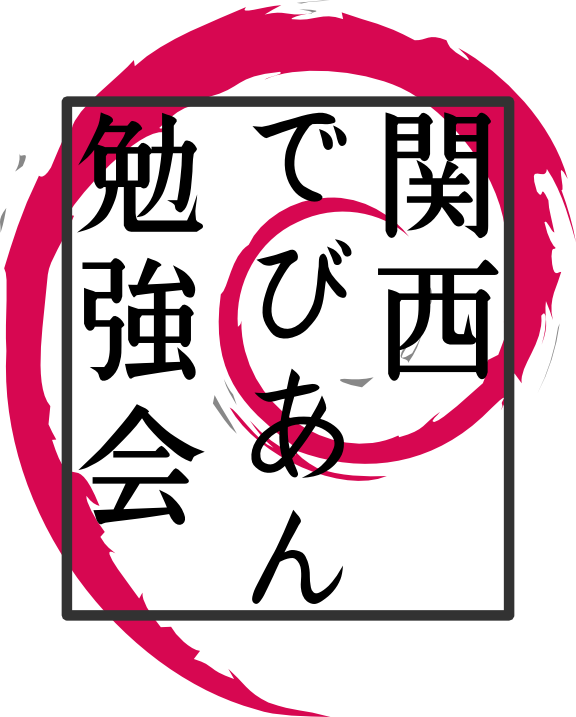
\includegraphics{image200802/kansaidebianlogo.png}
\end{center}

\begin{flushright}
\hfill{}関西 Debian 勉強会担当者 山下 尊也\\
\hfill{}\debmtgyear{}年\debmtgmonth{}月\debmtgdate{}日
\end{flushright}

\thispagestyle{empty}
\end{titlepage}

\dancersection{Introduction}{山下 尊也}
 
 関西 Debian 勉強会はDebian GNU/Linux のさまざ
 まなトピック(新しいパッケージ、Debian 特有の機能の仕組、Debian 界隈で起
 こった出来事、などなど)について話し合う会です。

 目的として次の三つを考えています。
 \begin{itemize}
  \item MLや掲示板ではなく、直接顔を合わせる事での情報交換の促進
  \item 定期的に集まれる場所
  \item 資料の作成
 \end{itemize}

 それでは、楽しい一時をお楽しみ下さい。

\newpage

\begin{minipage}[b]{0.2\hsize}
 {\rotatebox{90}{\fontsize{80}{80}
{\gt 関西デビアン勉強会}}}
\end{minipage}
\begin{minipage}[b]{0.8\hsize}
\hrule
\vspace{2mm}
\hrule
\setcounter{tocdepth}{1}
\tableofcontents
\vspace{2mm}
\hrule
\end{minipage}

\dancersection{GIS on Debian GNU/Linux!}{清野 陽一}

\subsection{はじめに}
\subsubsection{社会的整備の進展}

\begin{itemize}
 \item 国際情勢
       \begin{itemize}
	\item 地図情報を電子化して扱おうという試みは1960年代ごろから始まってい
	      る。当初は研究目的。
	\item メインフレーム上ではなく、ワークステーションやパーソナルコンピュー
	      タの発達に伴い、1980年代頃からこれらのコンピュータ上で動かせるシ
	      ステムが普及し始める。
	\item 後述する地上観測衛星(ランドサット衛星1号機の打ち上げは1972年)や
	      スペースシャトルの運用により、リモートセンシングなどの活用が1970
	      年代より行われるようになる。
       \end{itemize}
 \item 日本国内
 \begin{itemize}
  \item 行政サイド \\
	日本においては、国土に関する数値情報の電子化
	\begin{quotation}
	 「平成7年1月の阪神・
	 淡路大震災の反省等をきっかけに、政府において、GISに関する本格的な
	 取組が始まった。」(国土地理院
	 GIS\footnote{\url{http://www.gsi.go.jp/GIS/whatisgis.html}}による) 
	\end{quotation}
	→国を挙げての政策実施。2002年の小泉内閣における「e-Japan重点計
	画-2002」の重点政策のうち、4番目の「行政の情報化及び公共分野にお
	ける情報通信技術の活用の推進」においてGISの推進が盛り込まれる。
	ex)国土地理院の数値地図(CD-ROM版)は平成9(1997)年頃から整備される
	ようになってきている。
  \item 建設サイド
	\begin{itemize}
	 \item CAD(Computer Aided Design)の普及
	 \item 電子納品・標準化
	 \item 建設省・国土交通省の後押し
	\end{itemize}
 \end{itemize}
\end{itemize}

\subsubsection{個人レベル}
\begin{itemize}
 \item Google Earth、NASA World Windなどの無料かつ高性能なデスクトップ地
       図ビューワーの登場 \\
       →"Google Earthショック"
 \item Google MapなどのWebマッピングサイト \\
       →MashUpが流行\\
       →空間情報を個人が扱う時代に。
\end{itemize}

\subsection{GISとは}
\subsubsection{定義}
\begin{itemize}
 \item 国土地理院\footnote{\url{http://www.gsi.go.jp/GIS/whatisgis.html}}の説明
       \begin{quotation}
	地理情報システム(GIS:Geographic Information System)は、地理的位置を手がかりに、位置に関する
	情報を持ったデータ(空間データ)を総合的に管理・加工し、視覚的に表示し、高度な分析や迅速な判断
	を可能にする技術である。 
       \end{quotation}
 \item GISポータルサイト
       \footnote{\url{http://www.gis.go.jp/contents/about/whatis/index.html}}の説
       明
       \begin{quotation}
	GIS(Geographic Information System:地理情報システム)とは、位置や空間に関する様々な情報を、コ
	ンピュータを用いて重ね合わせ、情報の分析・解析をおこなったり、情報を視覚的に表示させるシステム
	です。元々は専門的な分野での利用が一般的でしたが、最近では、私たちの生活の中での身近な利用へと
	、その活用範囲が広がってきています。 
       \end{quotation}
 \item 国土交通省国土計画局
       \footnote{\url{http://www.mlit.go.jp/kokudokeikaku/gis/aboutgis/index.html}}
       の説明
       \begin{quotation}
	位置や空間に関する情報をもったデータ(空間データ)を総合的に管理・加工し、視覚的に表示できる高
	度な分析や迅速な判断を可能にする技術です。 
       \end{quotation}
 \item ESRIジャパン社
       \footnote{\url{http://www.esrij.com/whatisgis/gis/index.shtml}}の説明
       \begin{quotation}
	GISとは、Geographic Information Systemの略で、広義には「実世界を空間的に管理することにより
	、より合理的な意思決定を行おうとするアプローチ全般」を意味しますが、狭義には、「空間情報を作成
	、加工、管理、分析、表現、共有するための情報テクノロジ」を意味します。 
       \end{quotation}
 \item インフォマティクス社
       \footnote{\url{http://www.informatix.co.jp/sis/aboutgis/aboutgis.html}}の
       説明
       \begin{quotation}
	GISとは、Geographical Information Systems(地理情報システム)の略で地図上に様々な情報を重ね
	合わせて表示・編集したり、分析するシステムのことをいいます。
       \end{quotation}
\end{itemize}

\begin{itembox}[c]{"GIS"と"GPS"の違いってわかる?}
混同している人を良く見かけます。GPS="Global Positioning System"の略。

全地球測位システム、汎地球測位システム。アメリカの衛星システム。元軍事用。

カーナビとか携帯電話に入っているヤツね。
\end{itembox}

\subsubsection{大別して2タイプ}
\begin{itemize}
 \item 管理系GIS
       \begin{itemize}
	\item 統合型・全庁型 \\
	      商用製品が主流。ラージスケール指向。分析も出来る。\\
	      →ESRI社ArcGIS、インフォマティクス社のSIS、MapInfo社のMapInfoなど。
	      \\
	      →実際、助成金などでお金がある人は、個人研究者でも導入する人は多
	      い。\\
	      →その場合、操作方法を知っていることで就職時のアドバンテージにも。
	\item 表示系:Google Earth、Google Mapみたいなモノ。
	\begin{itemize}
	 \item mapserver:WebGISサーバ
	       \footnote{\url{http://mapserver.gis.umn.edu/}}
	 \item ka-Map\footnote{\url{http://ka-map.maptools.org/}}
	\end{itemize}
	\item CADとの関係\\
	      設計・測量・建設・土木・防災と密接に連携\\
	      →境目が曖昧になってきている\\
	      →Autodesk(AutoCAD)社のオープンソースへの参入
       \end{itemize}
 \item 解析系GIS
       \begin{itemize}
	\item GRASS GIS\footnote{\url{http://grass.itc.it/}}\\
	      1980年代半ばから開発
	\item Quantum GIS\footnote{\url{http://www.qgis.org/}}\\
	      高機能なビューワ。簡単な解析機能も持つ。
	\item SAGA
	      GIS\footnote{\url{http://www.saga-gis.uni-goettingen.de/html/index.php}}\\
	      Release 2.0.1はGentoo LinuxのPortage用が用意されてるみ
	      たい。
	\item Mandara\footnote{\url{http://www5c.biglobe.ne.jp/~mandara/}}\\
	      Windows用のGISソフト。初心者向け。GISがどういうものかをてっとり早
	      く知りたい人にはお手軽かも。MS Excelとの連携も。
       \end{itemize}
\end{itemize}

\subsection{最近の話題}
\begin{itemize}
 \item OSGeo財団\footnote{\url{http://www.osgeo.org/node/271}}日本支部\footnote{\url{http://www.osgeo.jp/}}\\
       大阪市立大学や株式会社オークニーなどが中心
 \item 関西オープンソース2007におけるカンファレンス\footnote{\url{http://www.osgeo.jp/?page_id=8}}\\
       「特別企画:OSGeo.JP 創造都市を支えるオープンソース GISの最前線」
 \item 書籍の整備
       \begin{itemize}
	\item 『入門Webマッピング(\textit{Web Mapping Illustrated})』(2006年5月、
	      オライリー)\footnote{\url{http://www.oreilly.co.jp/books/4873112826/}}
	\item \textit{Open Source Gis: A Grass Gis Approach}(2007年末に3rd
	      Editionが出た、Springer)\footnote{\url{http://www.grassbook.org/}}
       \end{itemize}
\end{itemize}

\subsection{なぜDebian GNU/Linuxか?}
\subsubsection{Debian GNU/Linuxを選んだ同機(個人的経験)}
\begin{itemize}
 \item[★] オープンソースなソフトウェアが使いたかった。\\
       →高機能なプロプライエタリなソフトウェアは沢山あるが、高価!組織や補助金で導入した場合
	   はライセンスの問題が$\dots$。\\
	→プログラマブルなのもいいかも(勉強になるかも)
 \item[★] DebianGISのようなプロジェクトがある(最近は停滞気味?)
 \item[○] 初心者的に、パッケージの管理が楽そうだった(APT万歳!!)。
 \item[●] でも、使いこなせるなら他のディストリビューションでもOK?\\
	   →ソースコードは公開されてることが多いし、Debian GNU/Linuxじゃ
	   なきゃダメなバイナリというのは無いと思う。\\
	   →Windows上で使える環境も着々と進んできている。まだUnix/Linux
	   にアドバンテージがあるけど。\\
	   →MacOSはGISはあんまり得意じゃないかも$\dots$。
 \item[●] 海外ではMandrivaとか(かつてのArcheOSとか)Gentoo
	   Linux(Gentoo-GIS overlay Project \footnote{\url{http://gentoo-gis.sourceforge.net/}}なんての
	   がある。)などもよく利用されている模様。
 \item[●] 最近は人に勧めるとしたらUbuntuか$\dots$。(個人的に紹介実績有り(泣))
\end{itemize}

\subsubsection{Debian GNU/Linuxにおけるパッケージ、ライブラリなど}

DebianGIS\footnote{\url{http://wiki.debian.org/DebianGis}}のリストから

\begin{commandline}
Geospatial packages of core concern
    Meta-packages
        *education-geography task from debian-edu: DebianGIS recommends these additions: qgis, gmt, gdal, proj.
 (education-geography already depends on grass):
    Binary packages
        *PostGIS
            RDBMSのPostgreSQLの地理情報拡張
        *GDAL(Geospatial Data Abstraction Library 地理空間データ抽象化ライブラリ?)
            座標系(投影)変換ライブラリ
        *GRASS
        *QuantumGIS. Includes qgis-plugin-grass
        *Mapserver
        *GEOS
        *PROJ: proj-doc: there are PDF files available, perhaps those would be better?
        *Earth3D
        *gpsd
        *gpsdrive
        *gpx2shp
        *gpsman
        *gpsmanshp
        *gpstrans
        *gpsbabel
        *thuban
        *gmt
        *OpenSceneGraph
        *OpenThreads
        *Avce00 and E00compr
        *OGDI
        *OpenJUMP: in debian/contrib, because it depend on batik and sun jre. Work is being done to get batik into 
debian/main, and openjump to work with GNU Classpath. Packaged instead of JUMP
        *JTS
        *TerraLib
        *mapnik
        *marble
        *Viking: a GPS track editor and analyzer
        Useful packages to be packaged
        Sorted by approximate priority.
            Libraries and bindings
            *Python Shapelib binding
            *Python Cartographic Library (PCL)
            *Tcl Shapelib binding
            *Ruby Shapelib binding
        Desktop/Analysis/Database
            *Ossim: currently being worked on (Francesco Lovergine)
            *PostLBS: powerful routing solution for PostgreSQL/PostGIS
            *TerraView: powerful GIS based on TerraLib (already in Debian, but obsolete)
            *OpenModeller: species occurrence modelling software
            *r-spatial: R/GRASS interface for GRASS 6 and other spatial software for R
                R言語:統計処理。空間統計ライブラリ
            *garmin-utils: similar in scope and function to gpstrans, but works with modern serial Garmins. 
See also the NetBSD port
            *e-foto: aerial photogrammetry. See this unanswered post
        Data
        OpenStreetMap
            *OpenStreetmap: Useful for upcoming release of gpsdrive
            *josm: Java Open Street Map Editor
            *gosmore: viewer of OSM XML data such as the planet.osm
        Sample datasets
            * GRASS's Spearfish dataset
            * OSGeo's NC sample dataset
    Java
        *gvSIG (top priority)
        *uDig: User-friendly Desktop Internet GIS
        *GeoServer
        *Postgisdriver-JUMP: currently being worked on. Contrib - depends on jump
        *GeoTools: Java GIS Toolkit
        *Deegree2 and iGeoPortal: currently being worked on. Binary package structure not yet clear.
        *NASA World Wind (Java version): Needs JOGL and perhaps SUN Java
        *JOGL: Java
        *Kosmos Desktop GIS derived from OpenJUMP (an unofficial package available)
            For more info on the Java state in Debian, see the moving java to Debian/main page.
    Live Web Apps
        *PyWPS: Python Web Processing Service
        *OpenLayers, TileCache, FeatureServer (all from MetaCarta)
        *p.mapper (unofficial packages available
    3D Visualization
        *ParaView: Very useful for 3D rapresentation of GRASS rasters and vectors
        *Visual Terrain Project: proposed
        *VisIt: 3D visualization
        *X3D: modern version of VRML, various libs & apps
        *OpenDX: the open source version of IBM's Visualization Data Explorer. Uses the IBM Public License
        *MINI: proposed, needed for VTerrain
        *OpenProducer: proposed, useful for OpenSceneGraph
    Lower Priority
        *Shape file utilities, including ShapeChecker
        *http://www.primagis.fi/ map extension for Plone; it builds on top of Mapserver, 
Python Cartographic Library (PCL) and Cartographic Objects for Zope (ZCO)
        *OpenEV: currently being worked on (Alex Bodnaru); old version, based on gtk1; the new one, based on 
gtk2, is still unsuitable to packaging
        *MB-System: multibeam, interferometry, and sidescan sonar data processing (GPL)
        *PhpPgGIS: ITP #381974. Project apparently inactive
        *Open3D GIS: Requires FreeWRL, see http://sourceforge.net/projects/freewrl/.
 Project apparently dead? https://sourceforge.net/projects/open3dgis/
        *dxf2svg: also the reciprocal svg2dxf (depends on pstoedit)
        *JGrass: currently being worked on. Contrib - needs jdk1.4, several contrib packages. Currently being
 fused with uDig - better postpone packaging until settled down
\end{commandline}

この他にFOSS4G Toolkit CDやArcheOS(Mandrivaだったが最近Ubuntu化した)など
のLive CDもある。\\
→FOSS4G Toolkit CDはMandriva向けのRPMセットとして配布するのみとなったよ
うだ。

\subsection{空間データ}

★以前は必要とする者が自ら取得することが一般的であったが、最近では各種空間
データが整備されてきている。

\subsubsection{国内}
\begin{itemize}
 \item 国土地理院発行の各種数値地図(有償)\footnote{\url{http://www.gsi.go.jp/}}\\
       ただし、近年、情報公開により閲覧を目的としてデータの無償公開が進
       んでいる。\\
       ex)国土地理院数値地図(空間データ基盤)の閲覧(試験公開)
       \footnote{\url{http://sdf.gsi.go.jp/}}
 \item 電子国土ポータル\footnote{\url{http://portal.cyberjapan.jp/index.html}}\\
       各種地図の閲覧を主眼。精細なベクトルデータを提供。専用プラグイン
       を用いて各自がWeb地図作成を行える。
 \item 陸域観測技術衛星「だいち」(ALOS)\\
       宇宙航空研究開発機構(JAXA\footnote{\url{http://www.jaxa.jp/index_j.html}})
       が2006年1月24日に打ち上げた衛星の観測データ。有料?
\end{itemize}

「高精度で標高抽出を行うためのパンクロマチック立体視センサ(PRISM)、およ
び土地被覆の観測を高精度に行うための高性能可視近赤外放射計2型(AVNIR-2)、
昼夜の別なく、また天候によらず陸域の観測が可能なフェーズドアレイ方式Lバ
ンド合成開口レーダ(PALSAR)の3つの地球観測センサを搭載」

※2008年1月8日、予定した精度が取得できないのではないかとの報道
\footnote{\url{http://www.asahi.com/special/space/TKY200801090162.html}}
がなされたが、その後の調査により、同年同月16日、新たな方法を用いることで懸念されていた
問題は改善できるとの発表がなされた
\footnote{\url{http://www.jaxa.jp/press/2008/01/20080116_sac_daichi_j.html}}。

\subsubsection{地球規模}
\begin{itemize}
 \item スペースシャトル地形データ Shuttle Radar Topography Mission
       (SRTM)\\
       1994年より実験開始。現在主に利用されているのは2000年に行われた第3回実験
       によって取得されたデータ。11日間の飛行で両極を除く地上の陸地の約
       80%、全人口密集地の約95%をカバーするデータを取得した。

       NASAのFTPサイト\footnote{\url{ftp://e0srp01u.ecs.nasa.gov/srtm/}}よりデータをダ
       ウンロード可能。一部有料。

       DEM(Digital Elevation Model)の作成用
 \item ランドサット衛星画像 Landsat Imagery (TM,
       ETM+)\footnote{\url{http://www.eorc.jaxa.jp/hatoyama/satellite/satdata/landsat_j.html}}\\
       メリーランド大学
       \footnote{\url{http://glcfapp.umiacs.umd.edu:8080/esdi/index.jsp}}
       からデータをダウンロード可能。
       様々な波長の光の反射データ。リモートセンシング用。
 \item 商用衛星画像データ\\
       Google EarthやGoogle Mapなどでは高精細な商用衛星画像データが用い
       られている。Earthsat社やDigital Globe社、Bluesky社など。\\
       確かに解像度が高く利用価値は高いが、非常に高価なので、費用対効果を考えて利用されている。
\end{itemize}

★でも結局研究目的の場合などは、今でも自分達でデータを取得しなければな
らないことの方が多い(泣)。

★なので、いかに効率的に、必要とされり正確・詳細な空間データを取得するかが問題となる。

\subsection{おわりに}
\subsubsection{まとめ}
以前に比べて環境は格段に良くなっている。

特に、こちらから能動的に各種データの整備を要求・もしくは自ら多大なコスト
をかけて取得しなくても、次々と空間基盤データの整備が行われてきている。

表示系の地図サイトなどは個人レベルで管理・運用できる環境が整っている。\\
→皆さんもちょっと触ってみませんか?

\subsubsection{反省点}
今回はGISの概要を説明することで大半を消費してしまった。より具体的な話が
出来なかったのが悔やまれる。

しかし、実際に使ってみないと実感が湧かないのも事実。
また、具体的な課題がないと、なかなか触るきっかけもないかも。

\dancersection{DebianでPCクラスタを作ってみよう}{中尾 昌広}

\subsection{はじめに}
安価で高速な並列計算機システムであるPCクラスタを、Debianを使ってセットアッ
プする方法について説明します。

\subsubsection{PCクラスタとは何か?}
クラスタ(cluster) とは英語で「ブドウの房、同じものが群らがっている様」みたいな意味です。
つまり、PCクラスタとは、複数台のPCをブドウのように(LANケーブルで)相互接続して、それらを協調動作させるシステムのことです。

\begin{figure}[!htbp]
 \begin{center}
 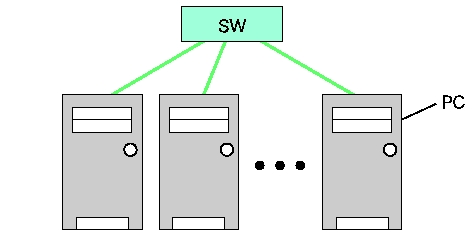
\includegraphics[width=82mm]{image200802/cluster.png}
  \caption{クラスタの概念図}
  \label{fig:ga-map}
 \end{center}
\end{figure}
\vspace{-3mm}

\subsubsection{PCクラスタをつくる理由}
高速な計算機環境が欲しいけど、スーパーコンピュータみたいな高価な専用並列計算機はとても買えない。
そこで、普通の電気屋で売っているようなPC をクラスタ化して、安価に並列計算環境を作ろう、ということが考えられました。

PCクラスタには大きく分けて、HA(High Availability)クラスタとHPC(High Performance Computing)クラスタがあります。
HAクラスタとは、高可用性を持つシステム、つまりサービスを止まりにくくすることを目的としたクラスタシステムです。
最近はWeb系のサーバでこのシステムがよく用いられています。
HPCクラスタとは、科学計算分野などでおいて、ものすごく時間のかかる処理を、複数台のPCに分散させて、
高速に結果を得ることを目的としたクラスタシステムです。
企業のメーカでも、車体や航空機を設計する際のシミュレーションなどに用いられています。

本資料とプレゼンでは基本的にHPCクラスタについての話ですが、HAクラスタに共通している点も多いはずです。

\subsubsection{DebianでPCクラスタを作る理由}
\begin{itemize}
\item Debianには数多くのPCクラスタ用ツールがある
\item PCクラスタのOSとして普通のDebianを利用するので、PCクラスタツール以外の有用なツールも数多く利用できる
\item コミュニティが活発(debian-usersで質問に答えてくれる人達は素晴らしい)
\item aptが楽
\end{itemize}

\subsection{PCクラスタの作り方}
並列計算ができるまでを目標として、PCクラスタシステムをセットアップする手順を説明します。
\begin{enumerate}
\item PCクラスタを構成する部品(PC、LANケーブル、スイッチングハブ)を用意し、それぞれ接続する
\item 用意したPCにDebian GNU/Linuxをインストールする
\item 自分が必要とするコンパイラと並列計算ライブラリをインストールする。
      並列計算ライブラリはmpichとPVMがよく用いられる。
      今回はmpichを使う
\begin{commandline}
 # aptitude install mpich-bin libmpich1.0-dev gcc g77 g++
\end{commandline}
      インストール後に並列計算に用いるホスト名(もしくはIPアドレス)を
      /etc/mpich/machines.LINUX記述する
\item クラスタ内ネットワークでは、速度重視のため暗号化なしで通信を行いた
      いので、rsh-serverとrsh-clientをインストールする
\begin{commandline}
 # aptitude install rsh-server rsh-client
\end{commandline}
      インストール後にrshを許可するホスト名(もしくはIPアドレス)を
      /etc/hosts.equivに記述する
\item NFSを使って/home以下の共有を行うと便利なため、PCクラスタを構成する
      PCの1台にnfs-kernel-serverをインストールする
\begin{commandline}
 # aptitude install nfs-kernel-server
\end{commandline}
      そして、nfs-kernel-serverをインストールしたPCの/etc/exportsに、ど
      のPCにNFSのサービスを許可するかの情報を記述する。
\begin{commandline}
 【/etc/exportsの例】
 /home   192.168.1.0/255.255.255.0(rw,async,no_subtree_check)
\end{commandline}
      /etc/exportsの変更後にNFSのサービスを再起動させる
\begin{commandline}
 # /etc/init.d/nfs-kernel-server restart
\end{commandline}
      そして、nfs-kernel-serverをインストールしたPC以外は、mountコマンド
      を用いてNFSサーバにマウントする
\begin{commandline}
 # mount -t nfs (NFSサーバ):/home /home
\end{commandline}
      以上で、PCクラスタの完成です。簡単です。
      意外かもしれませんが、並列計算ライブラリ以外は特殊なソフトウェアを用いていません。
      このように既存のソフトウェアを有効活用できる所が、PCクラスタの大きな特徴です。
 \item 並列計算用サンプルファイルが、
       /usr/share/doc/libmpich1.0-dev/examples/cpi.cにあるので、実行して
       みましょう。
\begin{commandline}
 $ mpicc cpi.c -o pi 【コンパイル】
 $ mpirun -np 5 pi   【実行】
\end{commandline}
       cpi.cは$\pi$の値を計算するプログラムです。
       mpiccというコマンドでC言語で書かれた並列計算プログラムのコンパイルが行えます。
       Fortranの場合はmpif77、C++の場合はmpicxxなどを用います。

       そして、mpirunというコマンドで、並列計算プログラムの実行が行えます。
       引数の-np以降はプロセス数を指定しています。
       また、並列計算に使用したいマシンを指定する際は、-machinefileというオプションを利用します。

\begin{commandline}
 $ mpirun -np 5 -machinefile hoge.txt pi
\end{commandline}

       この場合、hoge.txtに並列計算に使用したいホスト名を書くと、そのPC
       で並列計算が行われます。
\end{enumerate}

\subsection{クラスタで使うと便利なソフトウェア}
Gangliaという各ノードの負荷、生死をWebブラウザから確認できるソフトウェア。
日、週、月、年といった単位でクラスタ全体のロードアベレージの傾向も見ることができます。

\begin{figure}[htbp]
 \begin{center}
  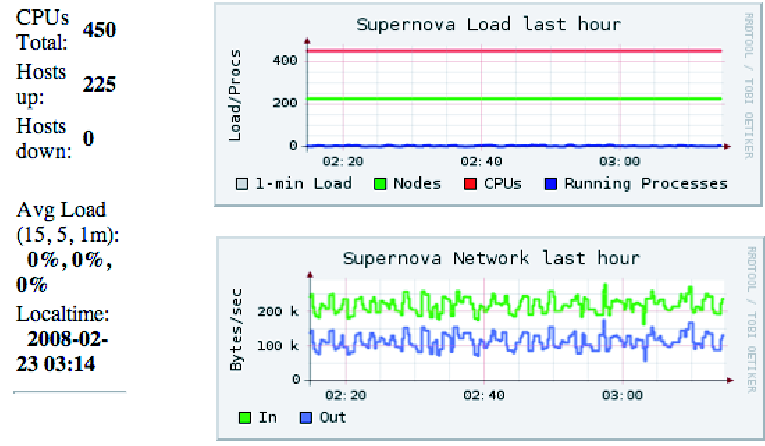
\includegraphics[width=100mm]{image200802/ganglia.png}
  \caption{Ganglia}
  \label{fig:ga-map}
 \end{center}
\end{figure}

\subsection{おわりに}
駆け足でクラスタの概要とセットアップ手順について説明しました。
Debianでクラスタを作るのは簡単だというのが伝われば幸いです。

\subsection{参考文献}
\begin{itemize}
\item 同志社大学知的システムデザイン研究室(\url{http://mikilab.doshisha.ac.jp/})
\item 超並列計算研究会(\url{http://www.is.doshisha.ac.jp/SMPP/})
\end{itemize}


\dancersection{資料作成基礎(TeX)}{山下 尊也}

\subsection{インストール}
今回、対象とするものは2008年2月21日現在のstableであるetchを対象とします。
私のセッションでは最小限の事しか述べないため、YaTeXなどを活用したい方は、
関連URLや東京エリア Debian 勉強会2007年12月の資料\footnote{whizzytexなど
を用いてプレビューさせるなど色々と技が載っています。}をご覧下さい。

\subsubsection{/etc/apt/sources.listの確認}

ノンフリーなものも使うため、/etc/apt/sources.listは以下のようにしておい
て下さい。

\begin{commandline}
deb http://ftp.debian.or.jp/debian/ etch main contrib non-free
\end{commandline}

\subsubsection{teTeX と pTeX一式のインストール}
\begin{commandline}
 $ sudo aptitude install ptex-bin
\end{commandline}

\subsubsection{奥村さんの新クラスファイルのインストール}
\begin{commandline}
 $ sudo aptitude install okumura-clsfiles
\end{commandline}

\subsubsection{dvipdfmxのインストール}
\begin{commandline}
 $ sudo aptitude install dvipdfmx
\end{commandline}

\subsubsection{Adobe Readerのインストール}
EtchのEvinceには日本語のフォントを埋め込んでない場合に文字が化けると言うバグ 
\footnote{いくやさんが修正したものを配布しています。
\url{http://ikuya.info/wiki/index.php?etchpackages} 
ただ、2008年2月22日現在のunstableでも、Evinceには、popplerの問題があり、
 \url{http://lists.debian.or.jp/debian-devel/200712/msg00000.html}これは、
AdobeとのCMAP問題に繋がるので、
Adobe Readerで見る事をお勧めします。
}
があるので、PDFを見るためにAdobe Readerをインストールする。

Adobe Readerの配布ページ
\footnote{\url{http://www.adobe.com/jp/products/acrobat/readstep2.html}}
にアクセスし、Adobe Readerのdebパッケージを取ってくる。

\begin{commandline}
 $ sudo dpkg -i AdobeReader_jpn-8.1.2-1.i386.deb
\end{commandline}

\subsubsection{CMAPのインストール}
\begin{commandline}
 $ sudo aptitude install cmap-adobe-japan1 cmap-adobe-japan2
\end{commandline}

\subsubsection{YaTeX(野鳥)のインストール}

エディタとしてEmacsを使っている人は、YaTeXと呼ばれる
\LaTeX 入力支援環境があるので、それを利用すれば良いでしょう。
\footnote{Emacsを使っていない方でも、VIM-\LaTeX
(\url{http://vim-latex.sourceforge.net/})や
KDE環境にKile(\url{http://kile.sourceforge.net/})という
\LaTeX を編集する環境があるようです。
}

\begin{commandline}
 $ sudo aptitude install yatex emacs21
\end{commandline}

文字コードは iso-2022-jp で統一しています\footnote{Windows 版と Linux 版
の ptex で共通して扱える文字コードにしたという経緯があります。ただし現状
Windows で全部できる状況ではありません。}。たとえば、emacs + yatex を使用
している場合で iso-2022-jp をデフォルトにするには、下記のような設定を
\texttt{.emacs} にかけばよいでしょう。

\begin{commandline}
(add-hook 'yatex-mode-hook
	  '(lambda () 
	     (progn 
	       (if (string-match "^/home/user/monthly-report/" default-directory)
		   (progn (set-buffer-file-coding-system 'iso-2022-jp)
			  (set-buffer-modified-p nil))))))
\end{commandline}

\texttt{.emacs}の例です。

\begin{commandline}
;;;;;;;;;;;;;;;;;;;;;;;;;;;;;;;;;;;;;;;;;;;;;;;;;;;;;;;;;;;;;;;;;;;;;;;;;
;; YaTeX
;;;;;;;;;;;;;;;;;;;;;;;;;;;;;;;;;;;;;;;;;;;;;;;;;;;;;;;;;;;;;;;;;;;;;;;;;
(setq auto-mode-alist
      (cons (cons "\\.tex$" 'yatex-mode) auto-mode-alist))
(autoload 'yatex-mode "yatex" "Yet Another LaTeX mode" t)
(defvar YaTeX-dvi2-command-ext-alist
  '(("xdvi" . ".dvi")
    ("ghostview\\|gv" . ".ps")
    ("acroread" . ".pdf")))
 (setq dvi2-command "acroread")
(setq dviprint-command-format "dvipdfmx `basename %s pdf`dvi")
;;; 色付け
(setq YaTeX-use-font-lock t)
(add-hook 'yatex-mode-hook
	  '(lambda () 
	     (progn 
	       (if (string-match "^/home/user/monthly-report/" default-directory)
		   (progn (set-buffer-file-coding-system 'iso-2022-jp)
			  (set-buffer-modified-p nil))))))
\end{commandline}

\subsection{文章の編集}

\LaTeX は最初は難しいと感じるかもしれませんが、基本は HTML と似たような
ものなので、まずはソースを読む事から始めてみると良いかもしれません。
\LaTeX についてさらに知りたい方は、
「[改訂第4版] \LaTeX 2美文書作成入門
(大型本) 奥村 晴彦 (著) 」
などの本を読む事をお勧めします。

\subsubsection{リポジトリからデータを取ってくる}
現在、関西 Debian 勉強会では、リポジトリの用意が出来ていないため、
東京エリア Debian 勉強会のリポジトリを借りている状態です。

\begin{commandline}
 $ sudo aptitude install git-core
 $ git-clone git://git.debian.org/git/tokyodebian/monthly-report.git
\end{commandline}

ドキュメントは p\LaTeX{}で作成しています。ファイル名として下記になってい
ます。(YYYY)(MM)は、年と月で、例えば2008年02月であれば 200802 です。

\begin{description}
 \item[debianmeetingresume(YYYY)(MM)-kansai.tex]
	    事前配布資料
 \item[debianmeetingresume(YYYY)(MM)-kansai-presentation.tex]
	    プレゼンテーション用 (prosperを利用)
 \item[image(YYYY)(MM)/]
	    画像ファイルなどの置き場
\end{description}

\subsubsection{基本部分の説明}

スタイルファイルは kansaimonthlyreport.sty パッケージを利用します。
このスタイルファイルは、東京エリア Debian 勉強会のスタイルファイルが
カラーなので、モノクロでも見やすいように編集しました。
今後、いろいろと手を加えていくと思います。

\begin{commandline}
\usepackage{kansaimonthlyreport} 
\end{commandline}

各担当部分は section として扱います。特別なコマンド dancersection で指定
します。形式は \texttt{dancersecion\{タイトル\}\{作者名\}}です。
その中で subsection や subsubsection を利用して文書を構成してくださ
い。

\begin{commandline}
 \dancersection{Debian 勉強会資料の準備の方法}{上川 純一}
 \label{sec:debmtg2007howtoprepare}
\end{commandline}

各担当部分は section として扱います。特別なコマンド dancersection で指定
します。形式は \texttt{dancersecion\{タイトル\}\{作者名\}}です。
その中で subsection や subsubsection を利用して文書を構成してくださ
い。

\begin{commandline}
 \dancersection{Debian 勉強会資料の準備の方法}{上川 純一}
 \label{sec:debmtg2007howtoprepare}
\end{commandline}

\subsubsection{画像ファイルの処理}

画面写真の画像を追加するときは、できるだけサイズの小さい png などを利用
してください。グラフなどの線画であれば、epsでかまいません。png であれば、 
ebb コマンドを利用してbounding box を作成してください。

\begin{commandline}
 ebb XXX.png
\end{commandline}

そして次のようにして文章に埋め込みます。

\begin{commandline}
\begin{figure}[!htbp]
\begin{center}
 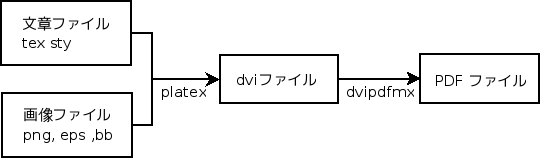
\includegraphics[width=120mm]{image200802/latex.png}
 \caption{\LaTeX で変換するイメージ}
 \label{fig:latex}
\end{center}
\end{figure}
\end{commandline}

\subsection{PDFへの変換}

変換の過程を簡単な図で示すと、図\ref{fig:latex}のようになります。

\begin{figure}[!htbp]
\begin{center}
 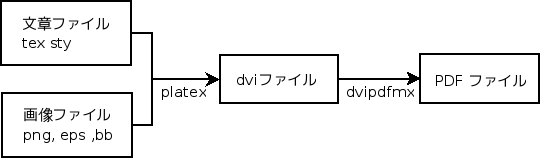
\includegraphics[width=120mm]{image200802/latex.png}
 \caption{\LaTeX で変換するイメージ}
 \label{fig:latex}
\end{center}
\end{figure}

コマンドで一つずつ変換をするならば、
\begin{commandline}
 $ platex debianmeetingresume200802-kansai.tex
 $ dvipdfmx debianmeetingresume200802-kansai.dvi
\end{commandline}

ですが、リポジトリから入手したものであれば、

\begin{commandline}
 $ make
\end{commandline}

\texttt{make}コマンドだけでファイルの更新があったファイルの変換などを
行なってくれます。

\dancersection{今後の予定}{山下 尊也}

\subsection{次回}
次回は、2008年03月23日に今回と同じく
港区民センター\footnote{\url{http://www.city.osaka.jp/shimin/shisetu/01/minato.html}}
梅にて行ないます。

\subsection{OSC Kansaiについて}
今年のOSC Kansaiの日程が決まりました。
7月18,19日(金・土)に行なわれます。

3月の中旬頃、OSC Kansaiのキックオフミーティングがあるので、
関西 Debian 勉強会も関係者が参加し、詳しい話を聞いてきます。

\subsection{KDRのおしらせ}
関西Debian勉強会の有志で
関西Debian勉強会とは独立した形で、
週に一度、読書会(KDR)を開いています。
詳しくは\url{http://qwik.jp/kdrweb/}をご覧下さい。
 
\printindex
 \cleartooddpage

 \begin{minipage}[b]{0.2\hsize}
  \rotatebox{90}{\fontsize{80}{80} {\gt 関西デビアン勉強会} }
 \end{minipage}
 \begin{minipage}[b]{0.8\hsize}

 \vspace*{15cm}
 \rule{\hsize}{1mm}
 \vspace{2mm}
 
\includegraphics[width=2cm]{image200502/openlogo-nd.eps}
 \noindent \Large \bf Debian 勉強会資料\\ \\
 \noindent \normalfont \debmtgyear{}年\debmtgmonth{}月\debmtgdate{}日 \hspace{5mm}  初版第1刷発行\\
 \noindent \normalfont 関西 Debian 勉強会 (編集・印刷・発行)\\
 \rule{\hsize}{1mm}
 \end{minipage}

\end{document}
